\documentclass[]{article}

\usepackage{graphicx}
\usepackage{subcaption}
\usepackage[hidelinks]{hyperref}
\hypersetup{colorlinks,urlcolor=blue, linkcolor=black}
\usepackage[tablegrid]{vhistory}
\usepackage{geometry}
\usepackage{fancyhdr}
\usepackage{lastpage}
\usepackage{lipsum}
\usepackage{pdflscape} % lscape pages in mostly portrait doc
% Coloured table entries
\usepackage[table]{xcolor}
% Colour legend
\usepackage{tikz}
\usetikzlibrary{fit}
% Float allows us to position images and tables more precisely
% [h] means put it roughly here, [H] means put it HERE!
\usepackage{float}
\usepackage{csvsimple} % Pull CSV files in to generate tables
\usepackage{listings} % Include for easy code listings
\usepackage[load=prefixed,load=abbr]{siunitx} % Simple SI units

\geometry{a4paper,total={170mm,257mm},left=25mm,top=25mm,bottom=30mm}
\parindent=0pt % disables indentation

\definecolor{codegreen}{HTML}{008000}
\definecolor{codepurp}{HTML}{881280}
\definecolor{codeblue}{HTML}{1A1AA6}

\lstdefinestyle{octavestyle}{
    %backgroundcolor=\color{backcolour},
    commentstyle=\color{codegreen},
    %keywordstyle=\color{magenta},
    numberstyle=\tiny\color{gray},
    stringstyle=\color{gray},
    %basicstyle=\ttfamily\footnotesize,
    basicstyle=\ttfamily\scriptsize,
    breakatwhitespace=false,
    breaklines=true,
    captionpos=b,
    keepspaces=true,
    %numbers=left,
    numbersep=5pt,
    showspaces=false,
    showstringspaces=false,
    showtabs=false,
    tabsize=2
}

\lstdefinestyle{xmlstyle}{
    %backgroundcolor=\color{backcolour},
    commentstyle=\color{codegreen},
    keywordstyle=\color{codepurp},
    numberstyle=\tiny\color{gray},
    stringstyle=\color{codepurp},
    moredelim=*[s][\color{codeblue}]{<}{>},
    %identifierstyle=\color{codeblue},
    %basicstyle=\ttfamily\footnotesize,
    basicstyle=\ttfamily\scriptsize,
    breakatwhitespace=false,
    breaklines=true,
    captionpos=b,
    keepspaces=true,
    %numbers=left,
    numbersep=5pt,
    showspaces=false,
    showstringspaces=false,
    showtabs=false,
    tabsize=2
}

\pagestyle{fancy}
\fancyhf{}
%\rhead{Overleaf}
\lhead{D-TACQ White Rabbit Concepts}
\lfoot{\textcopyright \space D-TACQ Solutions Ltd.}
\rfoot{Page \thepage \hspace{1pt} of \pageref{LastPage}}

%opening
\title{D-TACQ White Rabbit Concepts}
\author{D-TACQ Solutions}


\begin{document}

\maketitle
\thispagestyle{empty} % This suppresses the page number on titlepage
\begin{center}

\includegraphics{images/dtacq_logo_new}
\end{center}

\begin{abstract}
%\lipsum[1]
Overview of D-TACQ implementation of White Rabbit timing system, including clock derivation and trigger distribution.\\ \textcolor{red}{Red denotes placeholder sections that require expansion}
\end{abstract}

\begin{versionhistory}
    \vhEntry{1.0}{29/11/2021}{SR}{Created}
%    \vhEntry{2.0}{13/07/2021}{SR}{Added Test Setup section, more narrative}
%    \vhEntry{3.0}{13/07/2021}{SR|JM}{Minor tweaks; formatting}
%   \vhEntry{1.1}{23.01.04}{DP|JPW}{correction}
%   \vhEntry{1.2}{03.02.04}{DP|JPW}{revised after review}
\end{versionhistory}
\setcounter{table}{0} % Zeroes the table counter so the VerHist table isn't counted

\pagebreak

\tableofcontents

\pagebreak
\section{Glossary}
\begin{itemize}
	\setlength\itemsep{0pt}
	\item \href{https://www.timeanddate.com/time/international-atomic-time.html}{TAI} : Atomic Time
	\item WR : White Rabbit
	\begin{itemize}
		\item Precision network timing, clock shared with fixed phase on network
		\item Every UUT shares TAI with a time step size of 100 nS with an accuracy of < 1 nS
	\end{itemize}
	\item WRS : White Rabbit Switch
	\item PG : Pulse Generator
	\begin{itemize}
		\item Timed series of pulses, user programmed by STL.
	\end{itemize}
	\item STL : Signal Transition List
	\item WR Core Clock
	\begin{itemize}
		\item 250 MHz clock from the WR Core.
	\end{itemize}
	\item TIGA Clock
	\begin{itemize}
		\item Fixed integer divide on 250 MHz WR Core Clock. 10, 25 or 50 MHz.
		\item In a TIGA System this clock drives the Pulse Generators in the sites.
	\end{itemize}
	\item TAI Stamp
	\begin{itemize}
		\item External TRGIN timestamped against TAI 
	\end{itemize}
	\item WRTD
	\begin{itemize}
		\item White Rabbit Trigger Distribution: method for sharing trigger definitions on network.
	\end{itemize}
	\item WRTT
	\begin{itemize}
		\item White Rabbit Time Trigger: trigger edge generated at programmed TAI.
	\end{itemize}
	\item Derived CLKOUT
	\begin{itemize}
		\item Output clock on PG site LEMO, divided from input clock, synced to WR PPS.
	\end{itemize}
	\item Direct DO
	\begin{itemize}
		\item Logic output value, direct control from networked software knob.
	\end{itemize}
\end{itemize}
 
\section{Pulse per Second - PPS}
\subsection{Front Panel Outputs - acq400sync.opi}
\begin{itemize}
	\item SYNC.d0 carries the processed, 1 TIGA clock period wide, version of PPS. Not for customer use.
	\item SYNC.d1 carries the raw, 20 ms wide,  PPS pulse direct from the WR PTP Core. This is the true PPS which should be used for all comparisons, e.g. on scope measurements.
\end{itemize}

\begin{figure}[H]
	\centering
	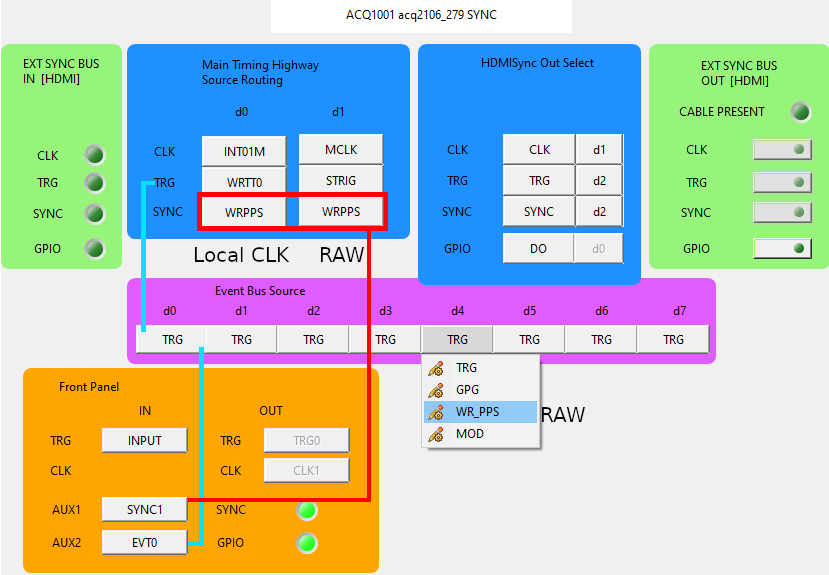
\includegraphics[height=0.5\textwidth]{images/evt_wr_pps_mod}
	\caption{CSS Sync OPI, RAW PPS to AUX1, WRTT0 to AUX2}
	\label{fig:syncopi}
\end{figure}

By default :
\begin{itemize}
	\item The RAW WR PPS from the WR PTP Core is available on AUX1 on the acq2106 front panel.
	\item WRTT0 is available on AUX2 on the acq2106 front panel.
\end{itemize}

Both of these outputs are used in the scope traces in further sections of this document.

\subsection{PPS Output Timing}\label{pps_out_timing}
\textcolor{red}{Skew introduced by getting the PPS off chip and discussion about pushing output onto IOB flip-flops.}

\section{WR Clock}
The embedded WR Core provides a 250 MHz clock (synchronized to global WR clock) and a pulse per second (PPS).\\

In general WR systems we use the included Si5326 clock synthesiser to dial up a subset of selected frequencies and "tune" this clock to result in near zero phase between the Si5326 clock and the WR clock.\\

In TIGA systems this was simplified to use an integer divide of the WR clock as the sample clock. This keeps everything within the FPGA without involving other devices on the motherboard.\\

We also take a copy of the WR PPS in order to provide synchronous divide on PG CLKOUTs in logic sites. This is only one clock wide and has an associated pipeline. This is accounted for in the design but this pulse should not be used by an end user.

\subsection{Si5326 Clock Tuning}
\textcolor{red}{We're specifying a fixed number of clock speeds for use as the box-wide WR clock driven from the Si5326. Typically 10, 20, 40 MHz}

\subsection{Synchronous Clock Divide on ADC Sites}
\textcolor{red}{Use the PPS on the sync bus to control clock divider reset. This allows us to divide the WR clock (10s of MHz) down to a speed that's suitable for the ADC}

\section{WR Trigger}
\subsection{Theory of Operation}
\textcolor{red}{Snapshot, add network delay, packetise, send WRTD message, program WRTT register, WRTT fires when time reached.}

\subsection{WRTD Utility Commands}

\subsubsection{Immediate}
\fbox{\texttt{set.site 11 wrtd\_txi}} - Trigger ASAP (network latency notwithstanding)
\subsubsection{On Next PPS}
\fbox{\texttt{set.site 11 wrtd\_txi --on\_next\_second=1}} - Trigger on next PPS
\subsubsection{At}
\fbox{\texttt{set.site 11 wrtd\_txa --at=+5:0}} - Trigger 5 seconds from now\\
\fbox{\texttt{set.site 11 wrtd\_txa --at=+5:25}} - Trigger 5 seconds and 25 nanoseconds from now\\
\fbox{\texttt{set.site 11 wrtd\_txa --at=+0:999999900}} - Trigger at 1 second, less 100 nanoseconds from now

%\subsubsection{Absolute}


\subsection{WRTD ID Labels}
\subsection{Accounting for Digitizer Trigger Setup Time and Multi-Rate Systems}

\pagebreak
\section{TAI in SPAD}
\textcolor{red}{Latch of WR\_CUR\_VERNR.0x218 in Agg is suboptimal. Although as an interesting side effect we get to see the acquisition time of the ADC in the timestamp. This is a nice way to demonstrate how ADC sampling aligns with trigger detection.}
Perhaps we should think about latching the TAI count with the sample clock. Bit ugly. This would require some extra control in the Aggregator; probably a new register.\\

We configure an ACQ423 box to include TAI time in the Scratchpad.\\
\texttt{set.site spad 1,8,0;run0 1;transient DEMUX=0}\\

Then we take a transient with a WRTT trigger, offload the data and look at the first few samples, followed by 200,000 samples in (1 second at ACQ423 sample rate). Below we're looking at sample number on the left and the bottom 28 bits of WR\_CURR\_VERNIER on the right.\\

\subsection{Trigger on PPS}

\textcolor{blue}{\texttt{set.site 11 wrtd\_txi --on\_next\_second=1}}

\begin{center}\begin{lstlisting}[language=bash,style=octavestyle]
hexdump -s $((0*4*24)) -e '16/4 "%08x " 1/4 "%10d " 7/4 "%08x " "\n"' shot_data | head -5 | awk '{ print $17,"\t",substr($19,2,16)}'
1 	 00001a1
2 	 0000269
3 	 0000331
4 	 00003f9
5 	 00004c1
hexdump -s $((199996*4*24)) -e '16/4 "%08x " 1/4 "%10d " 7/4 "%08x " "\n"' shot_data | head -5 | awk '{ print $17,"\t",substr($19,2,16)}'
199997 	 2625881
199998 	 2625949
199999 	 0000011
200000 	 00000d9
200001 	 00001a1
\end{lstlisting}\end{center}

\[	\textrm{40 MHz clock period }= 25\si{\ns}	\]
\[	1a1\textrm{ (hex)}= 417	\]
\[	417 \times 25 \si{\ns} = 10.425\si{\us}	\]

Acquisition time of an ACQ423 running at 200 kHz should be $\approx 5 \si{\us}$. Conclusion; the trigger has not arrived in time to be detected by the first clock.

\subsection{Trigger 200ns shy of PPS}

\textcolor{blue}{\texttt{set.site 11 wrtd\_txa --at=+0:999999800}}

\begin{center}\begin{lstlisting}[language=bash,style=octavestyle]
hexdump -s $((0*4*24)) -e '16/4 "%08x " 1/4 "%10d " 7/4 "%08x " "\n"' shot_data | head -5 | awk '{ print $17,"\t",substr($19,2,16)}'
1 	 00000d9
2 	 00001a1
3 	 0000269
4 	 0000331
5 	 00003f9
hexdump -s $((199996*4*24)) -e '16/4 "%08x " 1/4 "%10d " 7/4 "%08x " "\n"' shot_data | head -5 | awk '{ print $17,"\t",substr($19,2,16)}'
199997 	 26257b9
199998 	 2625881
199999 	 2625949
200000 	 0000011
200001 	 00000d9
\end{lstlisting}\end{center}

\[	d9\textrm{ (hex)}= 217	\]
\[	217 \times 25 \si{\ns} = 5.425\si{\us}	\]

Conclusion; with a 200ns setup time we catch the trigger on the first clock. In this configuration 100 ns did not seem to be enough... Let's compare with another mezzanine out of curiosity... None of the SARs should be any different.


\section{Pulse Generator}
\subsection{Trigger Debounce and Setup Time}

\section{Calibration}
\textcolor{red}{Slide the PPS against the PPS from the WRS until they match and call it a day. We should revisit this in concert with ideas referenced in Section \ref{pps_out_timing}.}

%\section{50 MHz TIGA Clock Example}
%
%\begin{figure}[H]
%	\centering
%	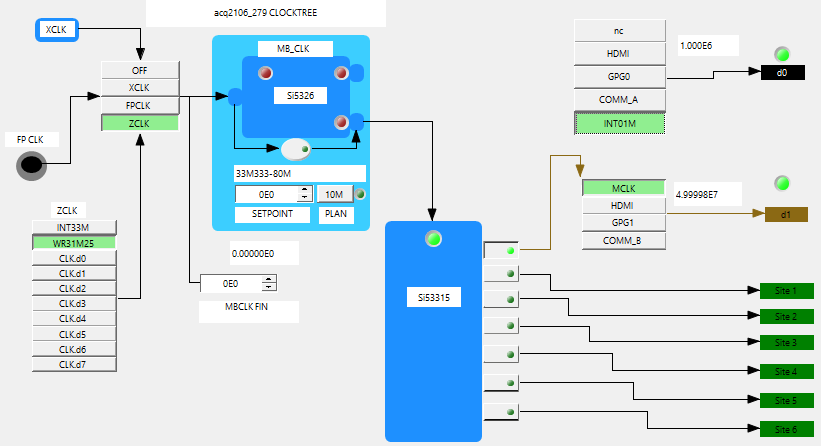
\includegraphics[height=0.4\textwidth]{images/50M_tiga_clk}
%	\caption{50 MHz TIGA Clock}
%	\label{fig:50M_clktree}
%\end{figure}
%
%N.B. The Si5326 clock synthesiser is not involved in a TIGA System. CLK.d1 is a fixed integer divide from the 250 MHz WR Core Clock.

\section{Miscellaneous Old Tests}
\subsection{Test Setup}

\begin{figure}[H]
	\centering
	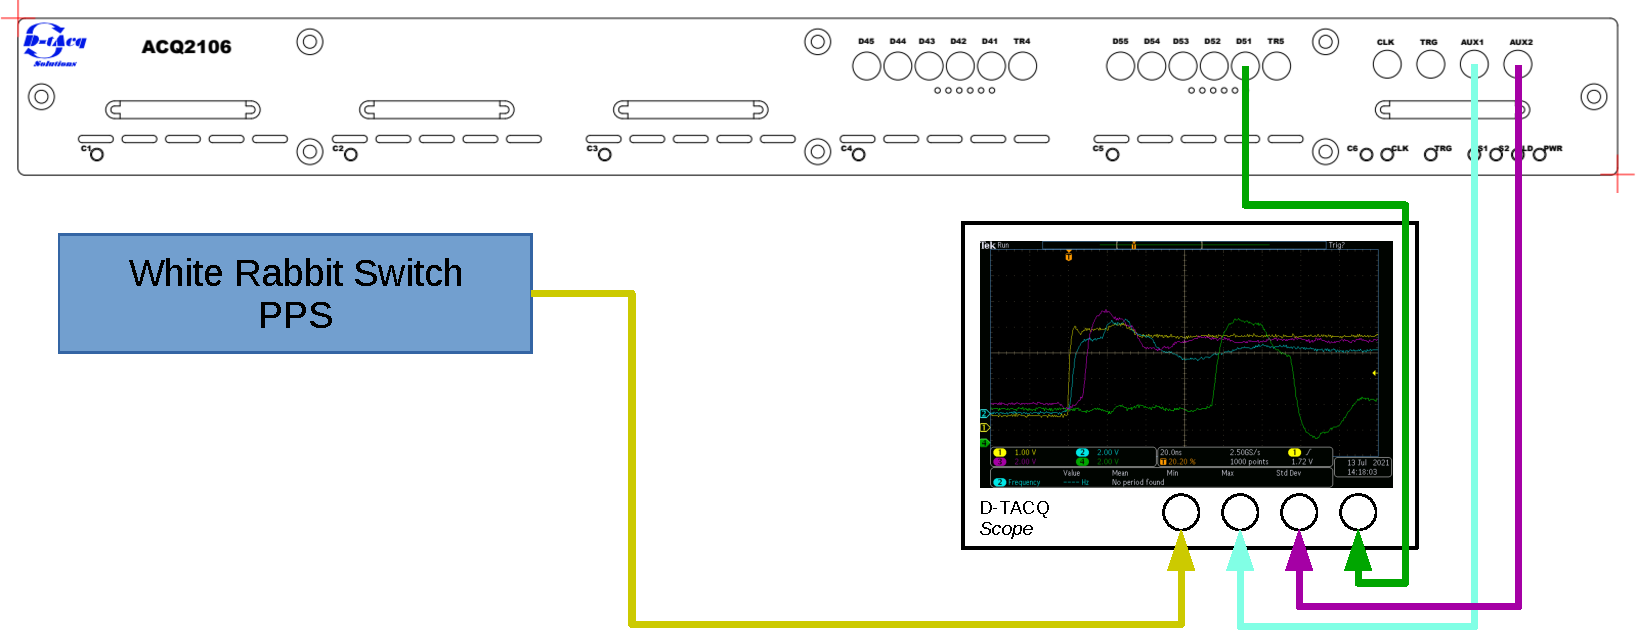
\includegraphics[height=0.4\textwidth]{images/system_diag}
	\caption{Test System Connections to Oscilloscope}
	\label{fig:sys_diag}
\end{figure}

%We're using the WR PPS to generate a WRTT at PPS + ~1s (details of control is outside the scope of this document). So the WRTT (magenta) in the scope trace is actually caused by a WRS PPS 1 second in the past.

Order of signals :
\begin{itemize}
	\setlength\itemsep{0pt}
	\item WR PPS from White Rabbit Switch (yellow)
	\item acq2106 connected to WRS via fiber-optic. WR synchronization take places giving us a local matched copy of PPS (cyan)
	\item We timestamp the rising edge of this PPS, add a delta of ~1s and tee-up a WRTT for this future time.
	\item The PG in Site 5 is programmed to trigger on the rising edge of WRTT0, producing the green output on PG1 (as per setup in Section \ref{pg_sect})
\end{itemize}

\begin{figure}[H]
	\centering
	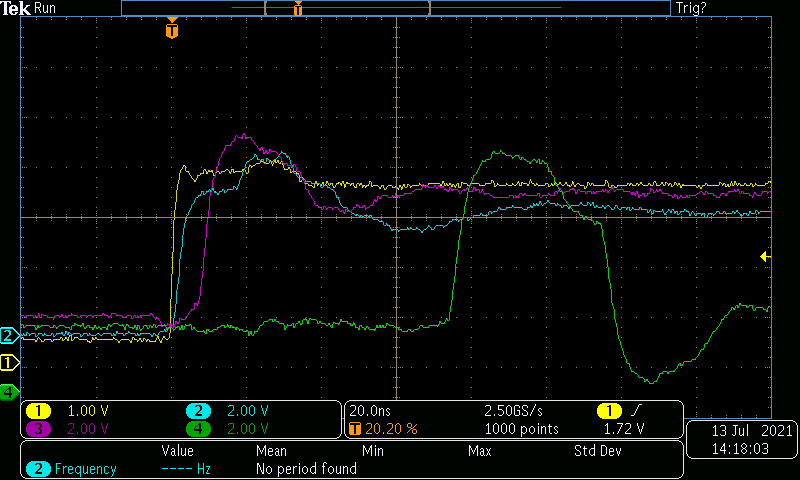
\includegraphics[height=0.5\textwidth]{images/wr_pps_ac_pps_wrtt0_pg}
	\caption{Yellow - WRS PPS; Cyan - acq2106 PPS; Magenta - WRTT0; Green - PG1 Site 5}
	\label{fig:pps_wrtt_pg}
\end{figure}

\begin{figure}[H]
	\begin{subfigure}{0.5\textwidth}
		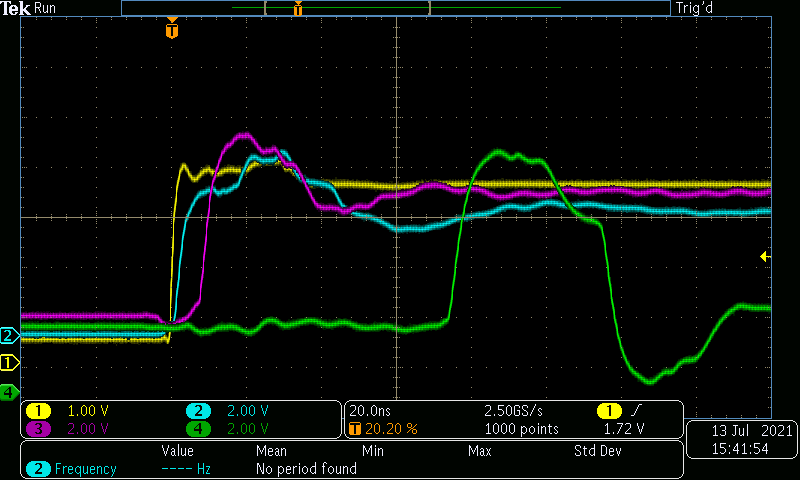
\includegraphics[width=0.9\linewidth]{images/wrts_source_add_pps_persist_wide}
		%\caption{Example D-TACQ Automated Test Setup with ACQ1001 and DAC Module}
		%\label{fig:cal_setup}
	\end{subfigure}
	\begin{subfigure}{0.5\textwidth}
		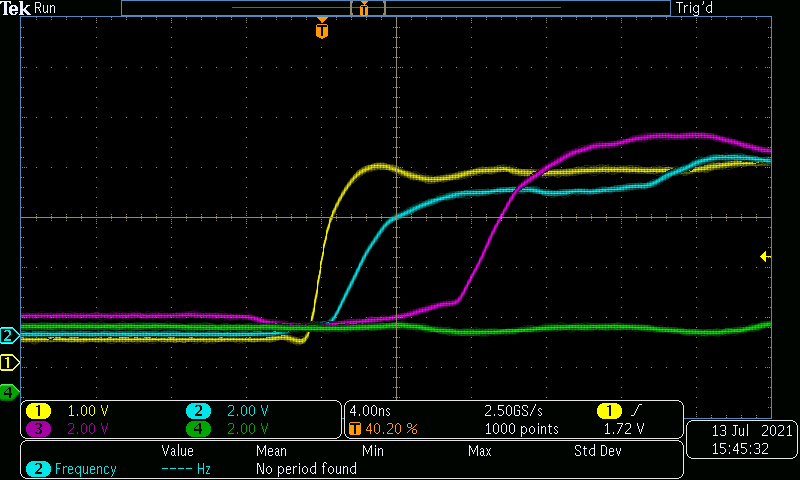
\includegraphics[width=0.9\linewidth]{images/wrts_source_add_pps_persist_zoom}
		%\caption{SYNC.opi Event Bus Source Selection}
		%\label{fig:cal_setup_photo}
	\end{subfigure}
	
	\caption{Identical to Figure \ref{fig:pps_wrtt_pg} but with a few minutes of scope persistence. Left - Wide, Right - Zoomed}
	\label{all_sigs_comp}
\end{figure}

\pagebreak
\subsection{PG Scope Trace and Configuration}\label{pg_sect}

We will need to ensure all our pipelines are correct in the PG configuration. However, what we have below is a PG clocked at 50 MHz showing a constant and steady phase offset relative to the WRTT0.

\begin{center}\begin{lstlisting}[language=bash,style=octavestyle]
	acq2106_279> cat pg_test
	#!/bin/sh
	
	export SITE=${SITE:-2}
	TSCALE=${TSCALE:-1}
	MODE=${1:-2}
	
	[ $TSCALE -ne 1 ] && echo Loading with timescaler=$TSCALE
	
	set.site $SITE gpg_enable 0
	set.site $SITE gpg_timescaler $TSCALE
	/usr/local/epics/scripts/gpg_monitor 1
	
	stl2gpg  /dev/acq400.$SITE.gpg <<EOF
	5,1
	7,0
	30,2
	40,0
	50,4
	60,0
	70,1f
	80,81
	90,00
	EOF
	
	# Set GPG to LOOP and Enable GPG
	set.site $SITE gpg_mode $MODE
	set.site $SITE gpg_enable 1
	
	acq2106_279> cat load-all-pg
	mode=${1:-0}
	for s in 4 5
	do
		set.site $s trg 1,0,1
		CSCALE=1 SITE=$s /mnt/local/pg_test $mode
	done
\end{lstlisting}\end{center}

\begin{figure}[H]
	\centering
	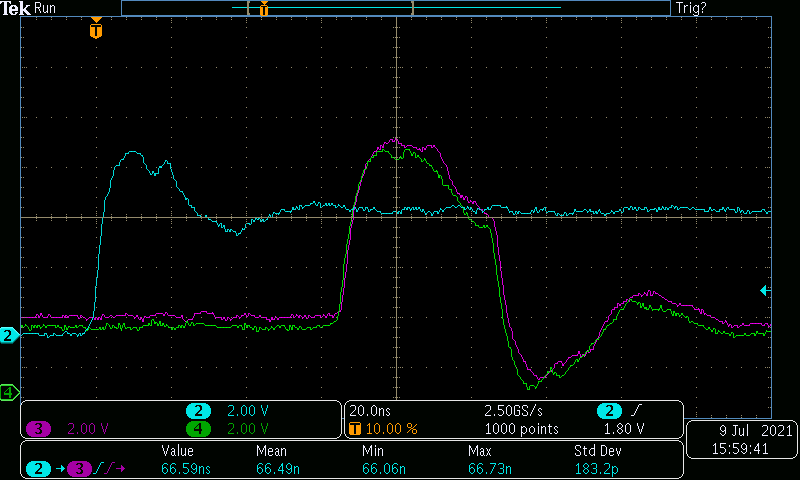
\includegraphics[height=0.5\textwidth]{images/WRTT_vs_PG1_S4_S5}
	\caption{Blue - WRTT; Green, Magenta - PG1 from Sites 4 and 5}
	\label{fig:wrtt_pg}
\end{figure}


\subsection{Derived CLKOUT Scope Trace}
\subsubsection{10 MHz CLKOUT from 10 MHz TIGA Clock}

\begin{figure}[H]
    \begin{subfigure}{0.5\textwidth}
        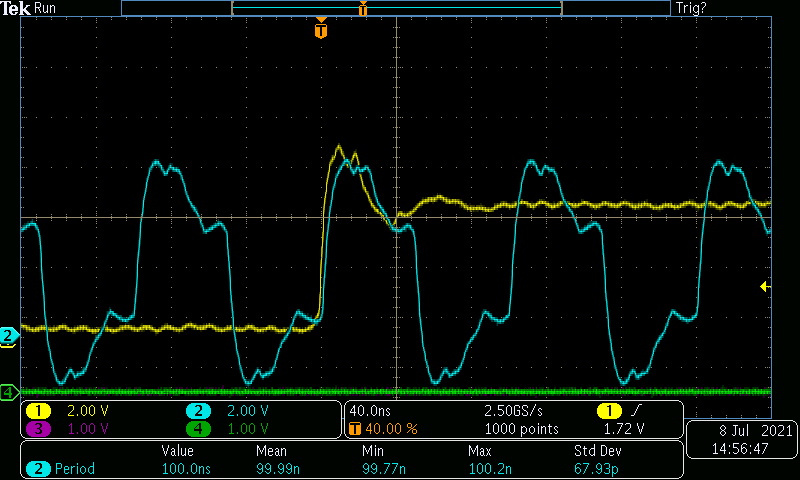
\includegraphics[width=0.9\linewidth]{images/WR_PPS_vs_10M_CLK_OUT_LEMO_PGSITE_WIDE}
        %\caption{Example D-TACQ Automated Test Setup with ACQ1001 and DAC Module}
        %\label{fig:cal_setup}
    \end{subfigure}
    \begin{subfigure}{0.5\textwidth}
        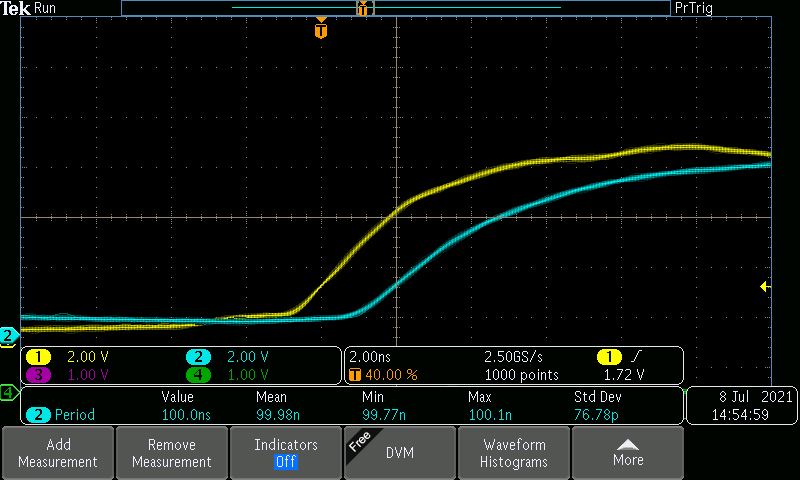
\includegraphics[width=0.9\linewidth]{images/WR_PPS_vs_10M_CLK_OUT_LEMO_PGSITE}
        %\caption{SYNC.opi Event Bus Source Selection}
        %\label{fig:cal_setup_photo}
    \end{subfigure}

    \caption{10 MHz Derived CLKOUT (no divide), relative to WR Core PPS. Left - Wide, Right - Zoomed}
    \label{10M_clkout}
\end{figure}

\subsubsection{1 Hz CLKOUT from 50 MHz TIGA Clock, large divide}
In site clock divider for derived CLKOUT expanded to 32-bits. Site 5 PG OPI showing 50,000,000 clkdiv.

\noindent\begin{minipage}{0.5\textwidth}% adapt widths of minipages to your needs
	\begin{lstlisting}[language=Octave,style=octavestyle]
	set.site 5 clk 1,1,1
	set.site 5 clkdiv 50000000

	set.site 5 bypass_trg 1 # Bypass Trigger Debounce
                          # preconditioned signal
	\end{lstlisting}
\end{minipage}%
\hfill%
\begin{minipage}{0.5\textwidth}
		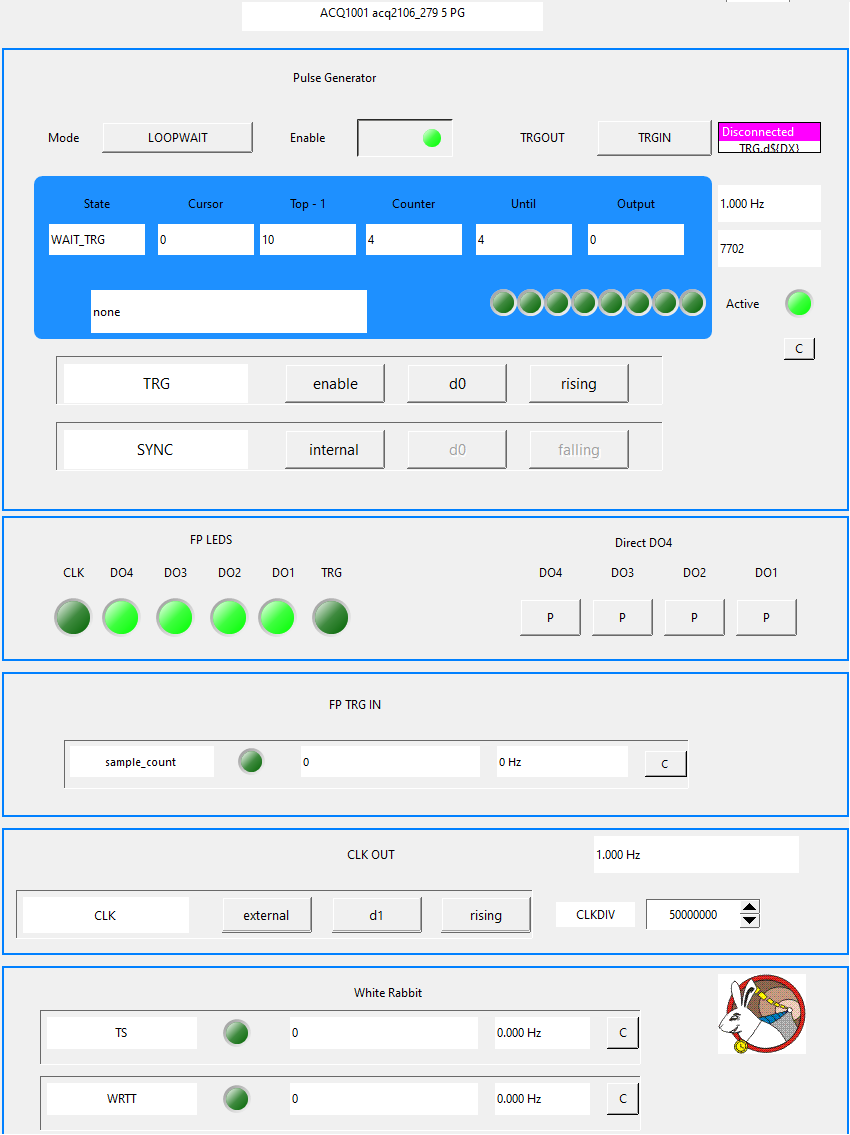
\includegraphics[height=\linewidth]{images/pg_with_50M_clkdiv}
%		\caption{Site 5 PG OPI showing 50,000,000 clkdiv}
\end{minipage}

%\begin{center}\begin{lstlisting}[language=bash,style=octavestyle]
%	set.site 5 clk 1,1,1
%	set.site 5 clkdiv 50000000
%	
%	set.site 5 bypass_trg 1 # Bypass Trigger Debounce
%	                        # preconditioned signal
%\end{lstlisting}\end{center}
%
%\begin{figure}[H]
%	\centering
%	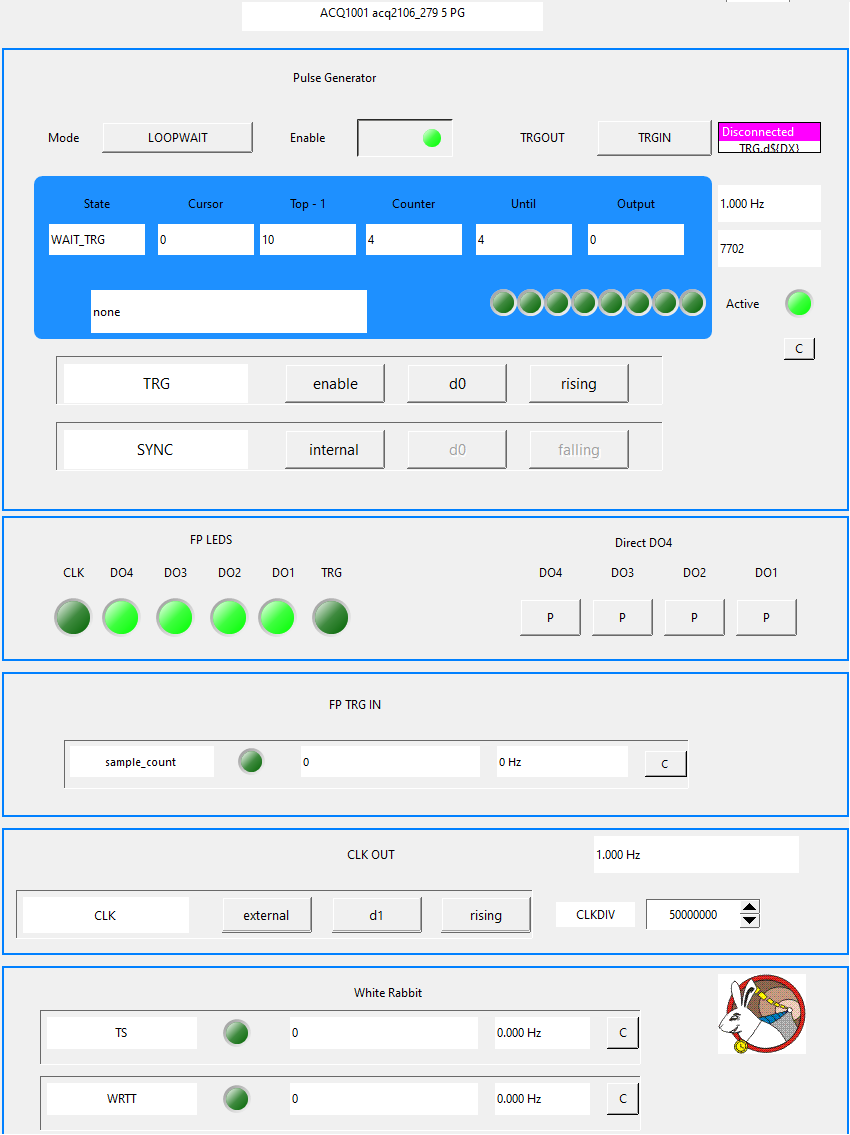
\includegraphics[height=0.4\textwidth]{images/pg_with_50M_clkdiv}
%	\caption{Site 5 PG OPI showing 50,000,000 clkdiv}
%	\label{fig:pg_big_clkdiv}
%\end{figure}

\begin{figure}[H]
	\begin{subfigure}{0.5\textwidth}
		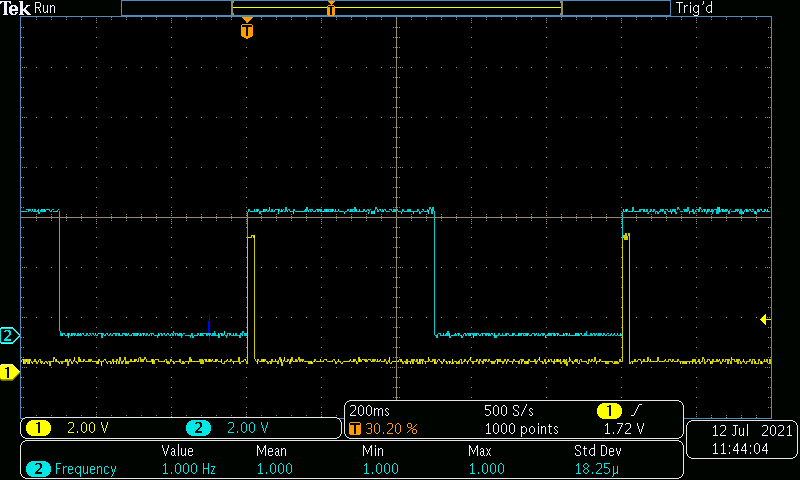
\includegraphics[width=0.9\linewidth]{images/50M_to_1Hz_wide}
		%\caption{Example D-TACQ Automated Test Setup with ACQ1001 and DAC Module}
		%\label{fig:cal_setup}
	\end{subfigure}
	\begin{subfigure}{0.5\textwidth}
		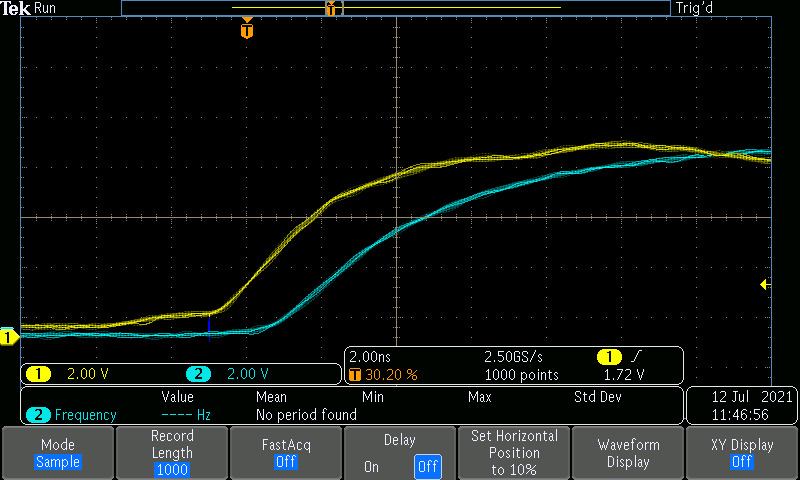
\includegraphics[width=0.9\linewidth]{images/50M_to_1Hz_zoom}
		%\caption{SYNC.opi Event Bus Source Selection}
		%\label{fig:cal_setup_photo}
	\end{subfigure}
	
	\caption{WR Core PPS vs 1 Hz Derived CLKOUT. Left - Wide, Right - Zoomed}
	\label{50M_clkout}
\end{figure}

%\begin{figure}[H]
%	\centering
%	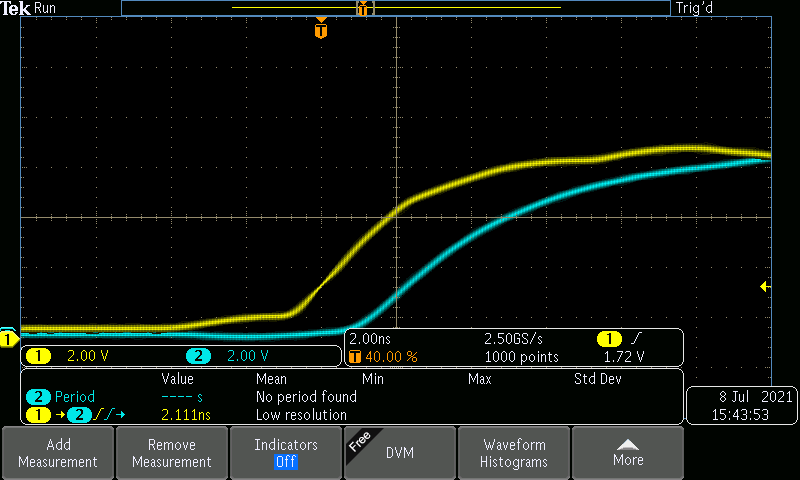
\includegraphics[height=0.5\textwidth]{images/PPS_vs_1Hz}
%	\caption{WR Core PPS vs 1 Hz Derived CLKOUT}
%	\label{fig:pps_vs_1}
%\end{figure}



%\section{Results - Before and After Changes}
%
%Note, not only the improved quality of the waveforms but also the more uniform DC offset leading to bunched channels rather than scattered channels.
%
%\begin{figure}[H]
%    \begin{subfigure}{0.5\textwidth}
%        
\includegraphics[width=0.9\linewidth]{images/dtacq_logo_new}
%        %\caption{Example D-TACQ Automated Test Setup with ACQ1001 and DAC Module}
%        %\label{fig:cal_setup}
%    \end{subfigure}
%    \begin{subfigure}{0.5\textwidth}
%        
\includegraphics[width=0.9\linewidth]{images/dtacq_logo_new}
%        %\caption{SYNC.opi Event Bus Source Selection}
%        %\label{fig:cal_setup_photo}
%    \end{subfigure}
%
%    \caption{Comparison of DAC Waveforms - 1 mV Sine - 2018 FPGA \& New 2021 FPGA}
%    \label{1mv_comp}
%\end{figure}

\end{document}
